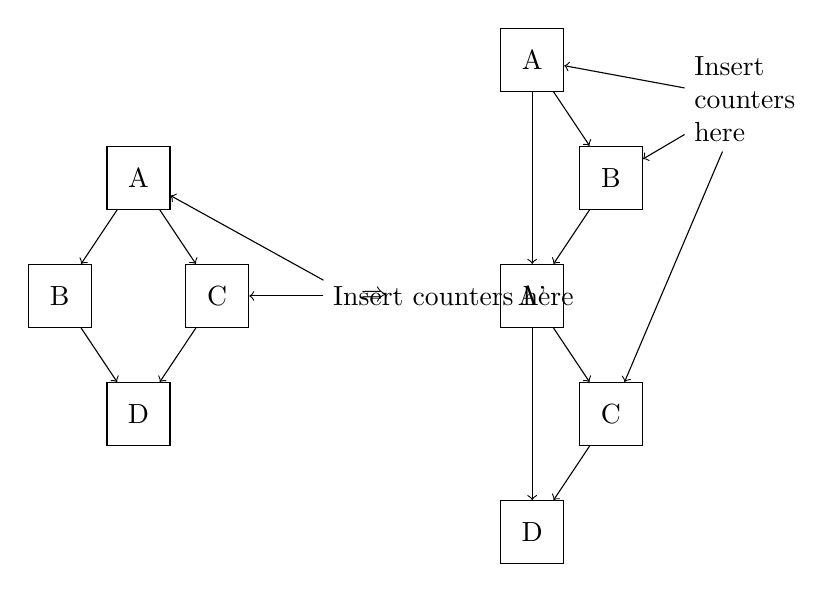
\begin{tikzpicture}
	\tikzstyle{box}=[minimum height=0.8cm, minimum width=0.8cm, rectangle, draw=black]

	\node[box] (a) at (0cm, 0cm) {A};
	\node[box] (b) at (-1cm, -1.5cm) {B};
	\node[box] (c) at (1cm, -1.5cm) {C};
	\node[box] (d) at (0cm, -3cm) {D};

	\draw[->] (a) -- (b);
	\draw[->] (a) -- (c);
	\draw[->] (b) -- (d);
	\draw[->] (c) -- (d);

	\visible<2>{
		\node (insert) at (4cm, -1.5cm) {Insert counters here};
		\draw[->] (insert.west)++(0cm, 0.2cm) -- (a);
		\draw[->] (insert.west) -- (c);
	}

	\visible<3->{
		\node at (3cm, -1.5cm) {$\Rightarrow$};

		\node[box] (a2) at (5cm, 1.5cm) {A};
		\node[box] (b2) at (6cm, 0cm) {B};
		\node[box] (a2') at (5cm, -1.5cm) {A'};
		\node[box] (c2) at (6cm, -3cm) {C};
		\node[box] (d2) at (5cm, -4.5cm) {D};

		\draw[->] (a2) -- (b2);
		\draw[->] (a2) -- (a2');
		\draw[->] (b2) -- (a2');
		\draw[->] (a2') -- (c2);
		\draw[->] (a2') -- (d2);
		\draw[->] (c2) -- (d2);
	}

	\visible<4>{
		\node[align=left] (insert) at (7.7cm, 1cm) {Insert\\counters\\here};
		\draw[->] (insert) -- (a2);
		\draw[->] (insert) -- (b2);
		\draw[->] (insert) -- (c2);
	}
\end{tikzpicture}
